\documentclass{article}

\usepackage{url}
\usepackage[hmargin=1.5in]{geometry}
\usepackage{amsmath}
\usepackage{amssymb}
\usepackage{amsthm}
\usepackage{eqnarray}
\usepackage{graphicx}
\usepackage[svgnames]{xcolor} %% for revisions
\usepackage{xparse} %% for squiggly underlines

%%\theoremstyle{definition}
%%\newtheorem{defn}{Definition}
\theoremstyle{plain}
\newtheorem{prop}{Proposition}

% convenience aliases
\newcommand{\maps}{\colon}

% symbology
\newcommand{\Z}{\mathbb{Z}}
\newcommand{\R}{\mathbb{R}}
\newcommand{\C}{\mathbb{C}}
\let\Re\relax
\DeclareMathOperator{\Re}{Re}
\newcommand{\laplace}{\mathcal{L}}
\newcommand{\series}[1]{\tilde{#1}}
\newcommand{\fracderiv}[3]{\partial^{#1}_{#2, #3}}
\DeclareMathOperator{\Ai}{Ai}

\title{Resurgence of the Airy function}
\author{Aaron Fenyes}

\begin{document}
\maketitle
\section{The Laplace transform}
\subsection{Analytic version}
\subsubsection{Regularity and decay properties}\label{reg-decay}
Let $\zeta$ be the standard coordinate on $\C$, and let $z \maps T^*\C \to \C$ be the fiberwise-linear map $d\zeta \mapsto 1$ (see ``The Geometry of the Laplace Transform'' in {\tt draft2}). The Laplace transform in $\zeta$ turns a function $\varphi$ on $\C$ into a function $\laplace_\zeta \varphi$ on $T^*\C$, defined on the cotangent space of $\zeta = \alpha$ by the integral
\[ \laplace_\zeta \varphi \big|_{\zeta = \alpha} = \int_{\Gamma_{\zeta, \alpha}} e^{-z \zeta}\,\varphi\;d\zeta, \]
where $\Gamma_{\zeta, \alpha}$ is the rightward ray starting at $\zeta = \alpha$ (compare {\tt draft2}). \textcolor{magenta}{We'll use the shorthand $\laplace_{\zeta, \alpha} f := \laplace_\zeta f \big|_{\zeta = \alpha}$ throughout this document [but maybe we should get rid of it].}

Let's say a function $f$ is in $O_{\zeta, \alpha \leftarrow}(g)$ or $O_{\zeta, \alpha \rightarrow}(g)$, respectively, if $|f| \lesssim g$ on some neighborhood of the starting point or infinite end of $\Gamma_{\zeta, \alpha}$. A function is {\em subexponential} along $\Gamma_{\zeta, \alpha}$ if it's in $O_{\zeta, \alpha \rightarrow}(e^{c\zeta})$ for all $c > 0$. Let $\mathcal{E}_{\zeta, \alpha}$ be the space of functions which are subexponential on $\Gamma_{\zeta, \alpha}$, integrable at the starting point, and locally integrable throughout. If $f$ is in $\mathcal{E}_{\zeta, \alpha}$, then $\laplace_{\zeta, \alpha} f$ is well-defined and holomorphic for $\Re(z) > 0$ on the part of $T^*\C$ that lies over $\Gamma_{\zeta, \alpha}$~\cite[\S 5.6]{diverg-resurg-i}.

The asymptotics of $f$ at the starting point of $\Gamma_{\zeta, \alpha}$ control the asymptotics of $\laplace_{\zeta, \alpha} f$ at the infinite end of $\Gamma_{z, 0}$. Once we see how this works for $\alpha = 0$, Section~\ref{translation} will do the rest. Let $F = \laplace_{\zeta, 0} f$. Equation~1.8 of \ref{laplace-tfm} shows\footnote{The argument cited still works in our generality. For holomorphic $f$, one can also use Equation 1.5 of {\em Borel-Laplace Transform and Asymptotic Theory} \textcolor{magenta}{(Sternin \& Shatalov)}.} that
\[ f \in O_{\zeta, 0 \leftarrow}(1) \quad\Longrightarrow\quad F \in O_{z, 0 \rightarrow}\left(\frac{1}{z}\right). \]
More generally, for $\tau > -1$ \textcolor{magenta}{[prove or cite]},
\[ f \in O_{\zeta, 0 \leftarrow}(\zeta^\tau) \quad\Longrightarrow\quad F \in O_{z, 0 \rightarrow}\left(\frac{1}{z^{1 + \tau}}\right). \]
Exact power law asymptotics relate similarly \textcolor{magenta}{[prove or cite]}:
\[ f \sim \zeta^\tau \text{ at the start of } \Gamma_{\zeta, 0} \quad\Longrightarrow\quad F \sim \frac{\Gamma(1+\tau)}{z^{1+\tau}} \text{ at the end of } \Gamma_{z, 0}. \]
\textcolor{magenta}{[The big-$O$ asymptotics dictionary is interesting, but we might not need it. Consider dropping.]}
\subsubsection{Action on integral operators}\label{L-int-op}
When $\varphi \in \mathcal{E}_\zeta$, you can use differentiation under the integral to show that~\cite[Theorem~1.34]{laplace-tfm}
\begin{equation}%%\label{id:L-mult}
\laplace_\zeta (\zeta^n \varphi) = \big({-\tfrac{\partial}{\partial z}}\big)^n \laplace_\zeta \varphi.
\end{equation}
for all integers $n \ge 0$. You can also use a 2d integration argument, akin to the one in \cite[Theorem~2.39]{laplace-tfm}, to show that $\fracderiv{-\lambda}{\zeta}{a} \varphi \in \mathcal{E}_\zeta$ and
\[ \laplace_{\zeta, a}\,\fracderiv{-\lambda}{\zeta}{a} \varphi = z^{-\lambda} \laplace_{\zeta, a} \varphi \]
for all $\lambda \in (0, \infty)$.

\color{violet}
When $\varphi$ is $n$ times differentiable, its $n$th derivative is in $\mathcal{E}$, and its zeroth through $(n - 1)$st derivatives extend continuously to zero, integration by parts gives the formula
\begin{align}\label{id:L-diff}
\laplace_\zeta \big(\tfrac{\partial}{\partial \zeta}\big)^n \varphi & = z^n \laplace_\zeta \varphi - \left[ \varphi\,z^{n-1} + \varphi'\,z^{n-2} + \varphi''\,z^{n-3} + \ldots + \varphi^{(n-1)} \right]_{\zeta = 0} \\
& = z^n\,\laplace\left( \varphi - \left[ \varphi + \varphi'\,\zeta + \tfrac{\varphi''}{2!}\,\zeta^2 + \ldots + \tfrac{\varphi^{(n-1)}}{(n-1)!}\,\zeta^{n-1} \right]_{\zeta = 0} \right). \nonumber
\end{align}
Note that if a function's derivative is subexponential, so is the function itself.\footnote{Say $f' \in O_{\zeta \to \infty}(e^{c\zeta})$. Then \[ \left|\int_0^Z f'\,d\zeta\right| \le \int_0^Z |f'|\,d\zeta \lesssim \int_0^Z e^{c\zeta}\,d\zeta = \tfrac{1}{c}(e^{cZ} - 1) \lesssim e^{cZ}.\] Now we know the integral on the left-hand side converges, implying that $f$ extends continuously to zero, with $|f - f_{\zeta = 0}| \lesssim e^{c\zeta}$.}
\subsection{Algebraic version}
\subsubsection{Definition}
Let $\mathcal{P}_\zeta$ be the vector space spanned by $\zeta^\alpha$ for $\alpha \in \R \smallsetminus \Z_{< 0}$. Note that $\mathcal{P}_\zeta \cap \mathcal{E}_\zeta$ is $\mathcal{P}_\zeta^{> -1}$, the subspace spanned by $\zeta^\alpha$ with $\alpha > -1$. Since
\[ \laplace_\zeta(\zeta^\alpha) = \Gamma(\alpha+1)\,z^{-(\alpha + 1)} \]
for all $\alpha > -1$, let's use the same formula to extend $\laplace_\zeta$ to all of $\mathcal{P}_\zeta$. This defines $\laplace_\zeta$ consistently on $\mathcal{E}_\zeta + \mathcal{P}_\zeta$.
\subsubsection{Action on differential operators}\label{L-diff-op-alg}
Observe that
\[ \laplace_\zeta(\zeta^{\alpha + 1}) = -\tfrac{\partial}{\partial z}\,\laplace_\zeta(\zeta^\alpha) \]
for $\alpha \neq -1$. This extends identity~\ref{id:L-mult} to all of $\mathcal{P}_\zeta$.

Observe that
\[ \laplace_\zeta\tfrac{\partial}{\partial \zeta}(\zeta^\alpha) = \begin{cases}
z\,\laplace_\zeta(\zeta^\alpha) & \alpha \neq 0 \\
0 & \alpha = 0,
\end{cases} \]
and that $0 = z\,\laplace_\zeta(1) - 1$. This recovers identity~\ref{id:L-diff} for any function in $\mathcal{P}_\zeta$ whose $n$th derivative is in $\mathcal{P}_\zeta^{> -1}$. Although the functions in $\mathcal{P}_\zeta^{< 0}$ are singular at zero, let's pretend they vanish at zero. With that convention, formula~\ref{id:L-diff} extends to all of $\mathcal{P}_\zeta$.

Now we have the results of Section~\ref{L-diff-op} for all functions in $\mathcal{E}_\zeta + \mathcal{P}_\zeta$. Identity~\ref{id:L-diff} is particularly simple when $\varphi$ has a {\em fractional power singularity} \textcolor{magenta}{[new terminology: when $\varphi$ is {\em slight}]} at $\zeta = 0$. By this, I mean that $\varphi$ can be written as $\varphi_\text{frac} + \varphi_\text{reg}$, where $\varphi_\text{frac} \in \mathcal{P}_\zeta$ has only non-integer exponents, and the zeroth through $(n-1)$st derivatives of $\varphi_\text{reg} \in \mathcal{E}_\zeta$ vanish at zero. Under this condition, all the initial value terms in the identity vanish, leaving
\[ \laplace_\zeta \big(\tfrac{\partial}{\partial \zeta}\big)^n \varphi = z^n \laplace_\zeta \varphi. \]
\color{black}
\subsection{Change of translation chart}\label{translation}
Define a new coordinate $\zeta_\alpha$ on $\C$ so that $\zeta = \alpha + \zeta_\alpha$. From the calculation
\begin{align*}
\laplace_{\zeta, a} \varphi & = \int_{\Gamma_{\zeta, \alpha}} e^{-z \zeta}\,\varphi\;d\zeta \\
& = \int_{\Gamma_{\zeta_\alpha, 0}} e^{-z(\alpha + \zeta_\alpha)}\,\varphi\;d\zeta_\alpha \\
& = e^{-\alpha z} \int_{\Gamma_{\zeta_\alpha, 0}} e^{-z\zeta_\alpha}\,\varphi\;d\zeta_\alpha \\
& = e^{-\alpha z} \laplace_{\zeta_\alpha, 0} \varphi,
\end{align*}
we learn that
\[ \laplace_{\zeta_\alpha, 0} \varphi = e^{\alpha z} \laplace_{\zeta, \alpha} \varphi. \]
\subsection{Rescaling of translation structure}
Let's rescale the translation structure of $\C$, expanding displacements by a factor of $\mu \in (0, \infty)$. The coordinate $\xi = \mu\zeta$ is a chart for the new translation structure. The corresponding frequency coordinate $x \maps T^*\C \to \C$ is given by $d\xi \mapsto 1$, so $x = \mu^{-1} z$. From the calculation
\begin{align*}
\laplace_{\xi, 0} \varphi & = \int_{\Gamma_{\xi, 0}} e^{-x\xi}\,\varphi\;d\xi \\
& = \int_{\Gamma_{\zeta, 0}} e^{-z \zeta}\,\varphi\;\mu\,d\zeta \\
& = \mu\,\laplace_{\zeta, 0} \varphi
\end{align*}
we learn that
\[ \laplace_{\xi, 0} \varphi = \mu\,\laplace_{\zeta, 0} \varphi. \]
Note that $\laplace_{\xi, 0}$ is defined in the new translation structure on $\C$, while $\laplace_{\zeta, 0}$ is defined in the old translation structure. We can still compare them, because they both turn complex-valued functions on $\C$ into holomorphic functions on $T^*\C$.
\section{Shifting integro-differential equations}\label{shifting}
Consider holomorphic functions on a simply connected open set that touches but doesn't contain $\zeta = 0$. A function is {\em regular} at $\zeta = 0$ if it extends holomorphically over that point. We'll say a function is {\em slight} at $\zeta = 0$ if it can be written as
\begin{equation}\label{eqn:slight-defn}
\zeta^{\alpha_1} f_1 + \ldots + \zeta^{\alpha_r} f_r + g
\end{equation}
where $f_1, \ldots, f_r$ are regular, $\alpha_1, \ldots, \alpha_r \in \R \smallsetminus \Z$, and $g, g', g'', \ldots$ go to zero at $\zeta = 0$.

Locally integrable slight functions play a special role in Laplace transform methods for linear differential equations. This is because differential equations in the frequency domain arise most naturally from integral equations in the spatial domain, but we'd like to work with differential equations in the spatial domain too. In the space of locally integrable slight functions, differential and integral equations enjoy their simplest equivalence.
\begin{prop}\label{prop:shifting}
When $\psi$ is slight and locally integrable at $\zeta = 0$,
\[ \left[ \sum_{k = 0}^n \big(\tfrac{\partial}{\partial \zeta}\big)^k \circ h_k + \sum_{k = 1}^m \fracderiv{-k}{\zeta}{0} \circ h_{-k} \right] \psi = 0, \]
if and only if
\[ \left[ \sum_{k = 1}^n \big(\tfrac{\partial}{\partial \zeta}\big)^{k-1} \circ h_k + \sum_{k = 0}^m \fracderiv{-k-1}{\zeta}{0} \circ h_{-k} \right] \psi = 0, \]
where $h_n, \ldots, h_{-m}$ are regular functions.
\end{prop}
To prove this result, we'll need a little background.

Each slight function has a unique {\em normal form}: an expression of the form (\ref{eqn:slight-defn}) where $\alpha_1, \ldots, \alpha_r$ are distinct modulo $\Z$ and $f_1, \ldots, f_r$ are non-vanishing at $\zeta = 0$. The {\em order} of a slight function is the smallest power $\alpha_k$ in its normal form. If there are no $\zeta^\alpha f$ terms, we say the order is $\infty$. A slight function vanishes at $\zeta = 0$ if and only if its order is positive, and it's locally integrable at $\zeta = 0$ if and only if its order is greater than $-1$.

Multiplication by a regular function and differentiation with respect to $\zeta$ both preserve the space of slight functions. Integration from $\zeta = 0$ preserves the space of locally integrable slight functions. Thus, in general, integro-differential operators with regular coefficients send locally integrable slight functions to slight functions. Each basic operation has a simple effect on a slight function's order. Multiplication by $\zeta^n f$, where $f$ is regular and non-vanishing at $\zeta = 0$, adds $n$ to the order. Differentiation and integration add $-1$ and $1$, respectively.
\begin{proof}[Proof of Proposition~\ref{prop:shifting}]
The reverse implication holds without any special condition on $\psi$, because $\tfrac{\partial}{\partial \zeta}\;\fracderiv{-1}{\zeta}{0}$ acts as the identity on all differentiable functions.

To prove the forward implication, rewrite the first equation in the statement as
\begin{equation}\label{eqn:diff-int-split}
\tfrac{\partial}{\partial \zeta} \left[ \sum_{k = 1}^n \big(\tfrac{\partial}{\partial \zeta}\big)^{k-1} \circ h_k \right] \psi = -\left[ h_0 + \sum_{k = 1}^m \fracderiv{-k}{\zeta}{0} \circ h_{-k} \right] \psi.
\end{equation}
The function
\[ \phi = \left[ \sum_{k = 1}^n \big(\tfrac{\partial}{\partial \zeta}\big)^{k-1} \circ h_k \right] \psi \]
is slight. Looking at the right-hand side of equation~\ref{eqn:diff-int-split}, we can see that $\phi'$ is slight and locally integrable, so its order is greater than $-1$. Hence, $\phi$ has positive order, which means it vanishes at $\zeta = 0$.

Integrating both sides of equation~\ref{eqn:diff-int-split}, we get
\[ \fracderiv{-1}{\zeta}{0}\;\tfrac{\partial}{\partial \zeta}\;\phi = -\left[ \fracderiv{-1}{\zeta}{0} \circ h_0 + \sum_{k = 1}^m \fracderiv{-k-1}{\zeta}{0} \circ h_{-k} \right] \psi. \]
Since $\fracderiv{-1}{\zeta}{0}\;\tfrac{\partial}{\partial \zeta}$ acts as the identity on functions that vanish at $\zeta = 0$, this simplifies to
\[ \phi = -\left[ \sum_{k = 0}^m \fracderiv{-k-1}{\zeta}{0} \circ h_{-k} \right] \psi, \]
which rearranges to the second equation in the statement.
\end{proof}
\section{The Airy equation}
\subsection{Basics}
The Airy equation is
\begin{equation}\label{eqn:airy}
\left[\big(\tfrac{\partial}{\partial y}\big)^2 - y\right] \psi = 0.
\end{equation}
One solution is given by the Airy function,
\[ \Ai(y) = \frac{i}{2\pi} \int_{\Gamma} \exp\left(-\tfrac{1}{3}t^3 + yt\right)\,dt, \]
where $\Gamma$ is a path that comes from $\infty$ at $120^\circ$ and goes to $\infty$ at $-120^\circ$.
\begin{center}
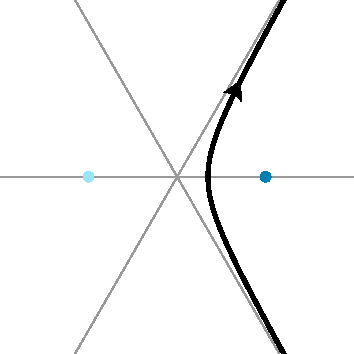
\includegraphics{figures/u_contour_3.pdf} \\[1em]
{\small The contour $\Gamma$ in the $u$ plane.}
\end{center}
With the substitution $t = 2uy^{1/2}$, we can rewrite the Airy integral as
\[ \Ai(y) = y^{1/2}\;\frac{i}{\pi} \int_{y^{-1/2} \Gamma} \exp\left[-\tfrac{2}{3}y^{3/2} \left(4u^3 - 3u\right)\right]\,du. \]
We've rescaled the contour by a factor of two, but it still approaches $\infty$ in the desired way. Note that $4u^3 - 3u$ is the third Chebyshev polynomial.
\subsection{Rewriting as a modified Bessel equation}
We can distill the most interesting part of the Airy function by writing
\[ \Ai(y) = \tfrac{1}{\pi\sqrt{3}}\,y^{1/2}\,K\big(\tfrac{2}{3} y^{3/2}\big), \]
where
\begin{equation}\label{integral:mod-bessel}
K(z) = i\sqrt{3} \int_{z^{-1/3}\Gamma} \exp\left[-z \left(4u^3 - 3u\right)\right]\,du.
\end{equation}
Saying that $\Ai$ satisfies the Airy equation is equivalent to saying that $K$ satisfies the modified Bessel equation
\begin{equation}\label{eqn:mod-bessel}
\left[z^2 \big(\tfrac{\partial}{\partial z}\big)^2 + z \tfrac{\partial}{\partial z} - \big[\big(\tfrac{1}{3}\big)^2 + z^2\big]\right] \varphi = 0.
\end{equation}
In fact, $K$ is the modified Bessel function $K_{1/3}$~\cite[equation~9.6.1]{dlmf}.

The method we'll demonstrate in Section~\ref{spatial} works for any differential equation
\[ \left[ P\big(\tfrac{\partial}{\partial z}\big) + z^{-1} Q\big(\tfrac{\partial}{\partial z}\big) + z^{-2} R(z^{-1}) \right] \varphi = 0, \]
where $P$ is a polynomial, $Q$ is a polynomial of one degree lower, and $R$ is an entire function. Let's put equation~\ref{eqn:mod-bessel} in that form:
\begin{equation}\label{eqn:reg-mod-bessel}
\left[ \big[ \big(\tfrac{\partial}{\partial z}\big)^2 - 1 \big] + z^{-1} \tfrac{\partial}{\partial z} - \big(\tfrac{1}{3}\big)^2 z^{-2} \right] \varphi = 0.
\end{equation}

\color{violet}
As we'll see in Section~\ref{asymp}, $K$ is in $O_{z \to \infty}(e^{-z})$. It'll be helpful to pull out the exponential decay factor and work instead with the function $K_1$ defined by $K = e^{-z} K_1$. Saying that $K$ satisfies equation~\ref{eqn:mod-bessel} is equivalent to saying that $K_1$ satisfies the equation
\begin{equation}\label{eqn:shifted-mod-bessel}
\left[z^2 \big(\tfrac{\partial}{\partial z} + 1\big)^2 + z \big(\tfrac{\partial}{\partial z} + 1\big) - \big[\big(\tfrac{1}{3}\big)^2 + z^2\big]\right] \varphi = 0.
\end{equation}
\color{black}
\subsection{Asymptotic analysis}
Equation~\ref{eqn:mod-bessel} has a regular singularity at $z = 0$ and an irregular singularity at $z = \infty$. From the general theory of such equations, we know that the space of trans-series solutions has a basis of trans-monomials
\[ \{ e^{-\alpha z} z^{-\tau_\alpha}\,\series{W}_\alpha \mid \alpha^2 - 1 = 0 \} \]
where the $\series{W}_\alpha$ are formal power series in $z^{-1}$ with no constant term. From equations 10.40.2 and 10.17.1 of \cite{dlmf}, we learn that $K \sim \left(\tfrac{\pi}{2}\right)^{1/2} e^{-z} z^{1/2}\,\series{W}_1$, with
\begin{equation}\label{bessel-asymp}
\series{W}_1 = z^{-1} - \frac{(\tfrac{1}{6})_1 (\tfrac{5}{6})_1}{2^1 \cdot 1!}\;z^{-2} + \frac{(\tfrac{1}{6})_2 (\tfrac{5}{6})_2}{2^2 \cdot 2!}\;z^{-3} - \frac{(\tfrac{1}{6})_3 (\tfrac{5}{6})_3}{2^3 \cdot 3!}\;z^{-4} + \ldots
\end{equation}

The holomorphic analysis in Section~\ref{spatial} will give us holomorphic solutions
\[ \{ e^{-\alpha z} z^{-\tau_\alpha}\,W_\alpha \mid \alpha^2 - 1 = 0 \}, \]
which seem analogous to the trans-monomials above. Borel summation makes the analogy precise. We'll see in Section~\ref{bessel-regularity} that each $z^{\tau_\alpha}\,W_\alpha$ is proportional to the Borel sum of $z^{\tau_\alpha}\,\series{W}_\alpha$.
\subsection{Going to the spatial domain}\label{spatial}
\color{violet}
\subsubsection{A good try at $\zeta = 0$}
Let's try to find a function $k_0$ with $K = \laplace_\zeta k_0$, which is unique if it exists~\cite[Theorem~1.23]{laplace-tfm}. If a function $\varphi$ satisfies the equation
\begin{equation}%%\label{eqn:spatial-mod-bessel}
\left[\big(\zeta^2 - 1\big) \big(\tfrac{\partial}{\partial \zeta}\big)^2 + 3\zeta \tfrac{\partial}{\partial \zeta} + \big[1 - \big(\tfrac{1}{3}\big)^2\big]\right] \varphi = 0,
\end{equation}
its Laplace transform $\varphi = \laplace_\zeta \varphi$ satisfies the equation
\begin{align*}
\left[\big({-\tfrac{\partial}{\partial z}}\big)^2 - 1\right] \Big(z^2 \varphi - \big[\varphi\,z + \varphi'\big]_{\zeta = 0}\Big) + 3\big({-\tfrac{\partial}{\partial z}}\big)\big[z\varphi - \varphi\big]_{\zeta = 0} + \big[1 - \big(\tfrac{1}{3}\big)^2\big] \varphi & = 0 \\
\big(\tfrac{\partial}{\partial z}\big)^2 \big[z^2 \varphi\big] - \Big(z^2 \varphi - \big[\varphi\,z + \varphi'\big]_{\zeta = 0}\Big) - 3\big(\tfrac{\partial}{\partial z}\big)\big[z\varphi\big] + \big[1 - \big(\tfrac{1}{3}\big)^2\big] \varphi & = 0 \\
\Big[2 + 4z\tfrac{\partial}{\partial z} + z^2\big(\tfrac{\partial}{\partial z}\big)^2\Big]\varphi - \Big(z^2 \varphi - \big[\varphi\,z + \varphi'\big]_{\zeta = 0}\Big) - 3\Big[1 + z\tfrac{\partial}{\partial z}\Big]\varphi + \big[1 - \big(\tfrac{1}{3}\big)^2\big] \varphi & = 0,
\end{align*}
which simplifies to
\begin{equation}\label{eqn:inhomog-mod-bessel}
\left[z^2 \big(\tfrac{\partial}{\partial z}\big)^2 + z \tfrac{\partial}{\partial z} - \big[\big(\tfrac{1}{3}\big)^2 + z^2\big]\right] \varphi = -\big[\varphi\,z + \varphi'\big]_{\zeta = 0}.
\end{equation}
Since we want $\laplace_\zeta k_0$ to satisfy equation~\ref{eqn:mod-bessel}, which is the homogeneous version of equation~\ref{eqn:inhomog-mod-bessel}, we might guess that $k_0$ is a solution of equation~\ref{eqn:spatial-mod-bessel} that vanishes through first order at $\zeta = 0$. Unfortunately, this would force $k_0$ to be zero.
\color{black}
\subsubsection{The big idea}\label{big-idea}
We're going to look for functions $v_\alpha$ whose Laplace transforms $\laplace_{\zeta, \alpha} v_\alpha$ satisfy equation~\ref{eqn:reg-mod-bessel}. We'll succeed when $\alpha^2 - 1 = 0$, and we'll see that $K$ is a scalar multiple of $\laplace_{\zeta, 1} v_1$.

We can see from Section~\ref{L-int-op} that $\laplace_{\zeta, \alpha} v$ satisfies the differential equation~\ref{eqn:reg-mod-bessel} if and only if $v$ satisfies the integral equation
\begin{equation}\label{int-eq:spatial-mod-bessel}
\left[ \big[ \zeta^2 - 1 \big] - \fracderiv{-1}{\zeta}{\alpha} \circ \zeta - \big(\tfrac{1}{3}\big)^2 \fracderiv{-2}{\zeta}{\alpha} \right] v = 0.
\end{equation}
It's tempting to differentiate both sides of this equation until we get
\begin{equation}\label{diff-eq:spatial-mod-bessel}
\left[ \big(\tfrac{\partial}{\partial \zeta}\big)^2 \circ \big[ \zeta^2 - 1 \big] - \tfrac{\partial}{\partial \zeta} \circ \zeta - \big(\tfrac{1}{3}\big)^2 \right] v = 0,
\end{equation}
which is easier to solve. Unfortunately, a solution of equation~\ref{diff-eq:spatial-mod-bessel} won't satisfy equation~\ref{int-eq:spatial-mod-bessel} in general. However, as we learned in Section~\ref{shifting}, a solution of equation~\ref{diff-eq:spatial-mod-bessel} {\em will} satisfy equation~\ref{int-eq:spatial-mod-bessel} if it's slight and locally integrable at $\zeta = \alpha$.

This is great news, because equation~\ref{diff-eq:spatial-mod-bessel} has a regular singularity at each root of $\zeta^2 - 1$, and the Frobenius method often gives a slight solution at each regular singular point. We can see the regular singularities by moving the derivatives to the right:
\[ \left[ (\zeta^2 - 1) \big(\tfrac{\partial}{\partial \zeta}\big)^2 + 3\zeta \tfrac{\partial}{\partial \zeta} + \big[ 1 - \big(\tfrac{1}{3}\big)^2 \big] \right] v = 0. \]

In Sections \ref{pos-root}\,--\,\ref{neg-root}, we'll see this approach succeed. For each root $\alpha$, we'll find a solution $v_\alpha$ of equation~\ref{diff-eq:spatial-mod-bessel} which is slight and locally integrable at $\zeta = \alpha$. We know the function $\laplace_{\zeta, \alpha} v_\alpha$ will satisfy equation~\ref{eqn:reg-mod-bessel}, and we can even find its asymptotics from the order $\tau_\alpha$ of $v_\alpha$. We learned in Section~\ref{translation} that
\[ \laplace_{\zeta, \alpha} v_\alpha = e^{-\alpha z} V_\alpha \]
where $V_\alpha = \laplace_{\zeta_\alpha, 0} v_\alpha$ and $\zeta = \alpha + \zeta_\alpha$. We can see from Section~\ref{reg-decay} that $V_\alpha$ is asymptotic to a scalar multiple of $z^{-1 - \tau_\alpha}$ at $z = \infty$, so the further decomposition
\[ \laplace_{\zeta, \alpha} v_\alpha = e^{-\alpha z} z^{-\tau_\alpha} W_\alpha, \]
makes $W_\alpha$ is asymptotic to a scalar multiple of $z^{-1}$ at $z = \infty$.
\color{Peru}
\begin{align*}
\left[ \big(\tfrac{\partial}{\partial \zeta}\big)^2 \circ (\zeta - 1)(\zeta + 1) - \tfrac{\partial}{\partial \zeta} \circ \zeta - \big(\tfrac{1}{3}\big)^2 \right] v & = 0
\end{align*}
\color{Sienna}
\begin{align*}
\left[ \big[ 2 + 2(2\zeta) \tfrac{\partial}{\partial \zeta} + (\zeta^2 - 1) \big(\tfrac{\partial}{\partial \zeta}\big)^2 \big] - \big[ 1 + \zeta \tfrac{\partial}{\partial \zeta} \big] - \big(\tfrac{1}{3}\big)^2 \right] v & = 0 \\
\left[ (\zeta^2 - 1) \big(\tfrac{\partial}{\partial \zeta}\big)^2 + 3\zeta \tfrac{\partial}{\partial \zeta} + \big[ 1 - \big(\tfrac{1}{3}\big)^2 \big] \right] v & = 0 \\
\left[ (\zeta - 1)(\zeta + 1) \big(\tfrac{\partial}{\partial \zeta}\big)^2 + 3\zeta \tfrac{\partial}{\partial \zeta} + \big[ 1 - \big(\tfrac{1}{3}\big)^2 \big] \right] v & = 0
\end{align*}
\color{black}
%%In terms of the coordinate $\zeta_\alpha$ with $\zeta = \alpha + \zeta_\alpha$, this equation is written
%%\begin{equation}\label{eqn:centered-mod-bessel}
%%\[ \left[ \big[ \zeta_\alpha (\zeta_\alpha + 2\alpha) + \alpha^2 - 1 \big] + \fracderiv{-1}{\zeta_\alpha}{0} \circ \big[ \zeta_\alpha + \alpha \big] - \big(\tfrac{1}{3}\big)^2 \fracderiv{-2}{\zeta_\alpha}{0} \right] w = 0. \]
%%\end{equation}
\subsubsection{Focus on $\zeta = 1$}\label{pos-root}
Let's find a solution of equation~\ref{diff-eq:spatial-mod-bessel} which is slight and locally integrable at $\zeta = 1$. Define a new coordinate $\zeta_1$ on $\C$ so that $\zeta = 1 + \zeta_1$. In this coordinate, equation~\ref{diff-eq:spatial-mod-bessel} looks like
\begin{equation}%%\label{diff-eq:spatial-mod-bessel-pos}
\left[\zeta_1(2 + \zeta_1) \big(\tfrac{\partial}{\partial \zeta_1}\big)^2 + 3(1 + \zeta_1) \tfrac{\partial}{\partial \zeta_1} + \big[1 - \big(\tfrac{1}{3}\big)^2\big]\right] v = 0.
\end{equation}
With another change of coordinate, given by $\zeta_1 = -2\xi_1$, we can rewrite equation~\ref{diff-eq:spatial-mod-bessel} as the hypergeometric equation
\begin{equation}\label{diff-eq:hypergeom-pos}
\left[\xi_1 (1 - \xi_1) \big(\tfrac{\partial}{\partial \xi_1}\big)^2 + 3(\tfrac{1}{2} - \xi_1) \tfrac{\partial}{\partial \xi_1} - \big[1 - \big(\tfrac{1}{3}\big)^2\big]\right] v = 0.
\end{equation}
Looking through the twenty-four expressions for Kummer's six solutions, we find one \cite[formula~15.10.12]{dlmf} which is manifestly slight and locally integrable at $\xi_1 = 0$:
\begin{alignat*}{2}
v_1 &=\;& \hphantom{-i\sqrt{2}}\,\xi_1^{-1/2} & F\big(\tfrac{1}{6}, \tfrac{5}{6}; \tfrac{1}{2}; \xi_1\big) \\
&=\;& -i\sqrt{2}\,\zeta_1^{-1/2} & F\big(\tfrac{1}{6}, \tfrac{5}{6}; \tfrac{1}{2}; -\tfrac{1}{2}\zeta_1\big)
\end{alignat*}
From the argument in Section~\ref{big-idea}, we know that $\laplace_{\zeta, 1} v_1$ satisfies equation~\ref{eqn:mod-bessel}, and can be written as $e^{-z} V_1$, where $V_1 = \laplace_{\zeta_1, 0} v_1$. Since $v_1$ has order $-1/2$, the decomposition $V_1 = z^{1/2} W_1$ makes $W_1$ asymptotic to a scalar multiple of $z^{-1}$ at $z = \infty$.
\subsubsection{Focus on $\zeta = -1$}\label{neg-root}
Let's find a solution of equation~\ref{diff-eq:spatial-mod-bessel} which is slight and locally integrable at $\zeta = -1$. In the rescaled coordinate from Section~\ref{pos-root}, this is the point $\xi_1 = 1$. Looking again through Kummer's table of solutions, we find another expression \cite[formula~15.10.14]{dlmf} which is manifestly slight and locally integrable at $\xi_1 = 1$:
\begin{alignat*}{2}
v_{-1} &=\;& (1-\xi_1)^{-1/2} & F\big(\tfrac{1}{6}, \tfrac{5}{6}; \tfrac{1}{2}; 1-\xi_1\big) \\
&=\;& \sqrt{2}\,\zeta_{-1}^{-1/2} & F\big(\tfrac{1}{6}, \tfrac{5}{6}; \tfrac{1}{2}; \tfrac{1}{2}\zeta_{-1}\big)
\end{alignat*}
where $\zeta_{-1}$ is the coordinate with $\zeta = -1 + \zeta_{-1}$. From the argument in Section~\ref{big-idea}, we know that $\laplace_{\zeta, -1} v_{-1}$ satisfies equation~\ref{eqn:mod-bessel}, and can be written as $e^z V_{-1}$, where $V_{-1} = \laplace_{\zeta_{-1}, 0} v_{-1}$. Since $v_{-1}$, like our other solution, has order $-1/2$, the same decomposition $V_{-1} = z^{1/2} W_{-1}$ makes $W_{-1}$ asymptotic to a scalar multiple of $z^{-1}$ at $z = \infty$.

In this example, $v_1$ and $v_{-1}$ happen to be related by a symmetry: the M\"{o}bius transformation that pulls $\zeta$ back to $-\zeta$. Kummer's solutions typically come from six different hypergeometric equations, which are related by the M\"{o}bius transformations that permute their singularities. In our case, though, exchanging $1$ with $-1$ keeps equation~\ref{diff-eq:spatial-mod-bessel} the same.

\color{DodgerBlue}
If we'd followed the routine from Section~\ref{pos-root}, rewriting equation~\ref{diff-eq:spatial-mod-bessel} in the coordinate $\zeta_{-1}$ and then rewriting it again in a more recognizable form, we would've arrived at the hypergeometric equation
\[ \left[\xi_{-1} (1 - \xi_{-1}) \big(\tfrac{\partial}{\partial \xi_{-1}}\big)^2 + 3(\tfrac{1}{2} - \xi_{-1}) \tfrac{\partial}{\partial \xi_{-1}} - \big[1 - \big(\tfrac{1}{3}\big)^2\big]\right] v = 0, \]
where $\zeta_{-1} = 2\xi_{-1}$. This is the same as what we'd get by substituting $\xi_{-1}$ for $\xi_1$ in Section~\ref{pos-root}! In other words, the holomorphic map that pulls $\xi_{-1}$ back to $\xi_1$
\color{black}
\color{violet}
\subsubsection{Success at $\zeta = 1$}\label{spatial-success}
Let's try instead to find a function $k_1$ with $K = \laplace_{\zeta, 1} k_1$ \textcolor{magenta}{[This would be called $K_1$ in our new notation.]}. Define a new coordinate $\zeta_1$ on $\C$ so that $\zeta = 1 + \zeta_1$. Since
\begin{align*}
\laplace_{\zeta_1, 0} k_1 & = e^z \laplace_{\zeta, 1} k_1 \\
& = e^z K \\
& = K_1,
\end{align*}
we want $\laplace_{\zeta_1} k_1$ to satisfy equation~\ref{eqn:shifted-mod-bessel}. Rewrite equation~\ref{eqn:spatial-mod-bessel} as
\begin{equation}\label{eqn:shifted-spatial-mod-bessel}
\left[\zeta_1(\zeta_1 + 2) \big(\tfrac{\partial}{\partial \zeta_1}\big)^2 + 3(\zeta_1 + 1) \tfrac{\partial}{\partial \zeta_1} + \big[1 - \big(\tfrac{1}{3}\big)^2\big]\right] \varphi = 0.
\end{equation}
If $\varphi$ satisfies equation~\ref{eqn:shifted-spatial-mod-bessel}, $\laplace_{\zeta_1} \varphi$ will satisfy an inhomogeneous version of equation~\ref{eqn:shifted-mod-bessel}, analogous to equation~\ref{eqn:inhomog-mod-bessel}. This time, though, there's a trick we can use to zero out the inhomogeneity. Equation~\ref{eqn:shifted-spatial-mod-bessel} has a regular singularity at $\zeta_1 = 0$, and one solution (up to scaling) is a holomorphic multiple of $\zeta_1^{-1/2}$.\footnote{\textcolor{magenta}{Explain how to see.}} That solution has a fractional power singularity at $\zeta_1 = 0$, as defined in Section~\ref{L-diff-op-alg}, so its Laplace transform in $\zeta_1$ satisfies equation~\ref{eqn:shifted-mod-bessel}.

Following this plan, let's find $k_1$ explicitly. Defining another coordinate $\xi$ on $\C$ so that $\zeta_1 = -2\xi$, we can rewrite equation~\ref{eqn:shifted-spatial-mod-bessel} as the hypergeometric equation
\begin{equation}\label{eqn:hypergeom}
\left[\xi(1 - \xi) \big(\tfrac{\partial}{\partial \xi}\big)^2 + 3(\tfrac{1}{2} - \xi) \tfrac{\partial}{\partial \xi} - \big[1 - \big(\tfrac{1}{3}\big)^2\big]\right] \varphi = 0.
\end{equation}
The hypergeometric function
\[ g_1 = F\big(\tfrac{2}{3}, \tfrac{4}{3}; \tfrac{3}{2}; \xi\big) \]
satisfies equation~\ref{eqn:hypergeom} by definition. It's not the solution we want, though, because it's holomorphic around $\xi = 0$. Formula~15.10.12 from \cite{dlmf} gives another solution,
\[ f_0 = \xi^{-1/2} F\big(\tfrac{1}{6}, \tfrac{5}{6}; \tfrac{1}{2}; \xi\big), \]
which is a holomorphic multiple of $\xi^{-1/2}$ near $\xi = 0$. By the argument above, $F_0 = \laplace_{\zeta_1} f_0$ satisfies equation~\ref{eqn:shifted-mod-bessel}. This suggests that a constant multiple of $f_0$ is our desired $k_1$. The power series~\cite[equation~15.2.1]{dlmf}
\[ f_0 = \xi^{-1/2} + \frac{(\tfrac{1}{6})_1 (\tfrac{5}{6})_1}{(\tfrac{1}{2})_1 \; 1!}\;\xi^{1/2} + \frac{(\tfrac{1}{6})_2 (\tfrac{5}{6})_2}{(\tfrac{1}{2})_2 \; 2!}\;\xi^{3/2} + \frac{(\tfrac{1}{6})_3 (\tfrac{5}{6})_3}{(\tfrac{1}{2})_3 \; 3!}\;\xi^{5/2} + \ldots \]
converges near $\xi = 0$, showing that
\[ f_0 \in \xi^{-1/2} + O_{\xi \to 0}(\xi^{1/2}). \]
In terms of $\zeta_1$, we have
\[ f_0 \in -i \sqrt{2}\,\zeta_1^{-1/2} + O_{\zeta_1 \to 0}(\zeta_1^{1/2}). \]
Using the decay properties from Section~\ref{reg-decay}, we deduce that
\[ F_0 \in -i \sqrt{2\pi}\,z^{-1/2} + O_{z \to \infty}(z^{-3/2}). \]
Since we know that $F_0$ satisfies equation~\ref{eqn:shifted-mod-bessel}, this confirms that $F_0$ is a constant multiple of $K_1$, which is the only subexponential solution of equation~\ref{eqn:shifted-mod-bessel} (up to scaling). Comparing with series~\ref{bessel-asymp}, we see that $K_1 = \tfrac{i}{2}\,F_0$. We conclude that $K_1 = \laplace_{\zeta_1} k_1$ for
\[ k_1 = \tfrac{1}{\sqrt{2}}\,\zeta_1^{-1/2} F\big(\tfrac{1}{6}, \tfrac{5}{6}; \tfrac{1}{2}; -\tfrac{1}{2}\zeta_1\big). \]
\color{black}
\section{The Airy-Lucas equation}
\subsection{Basics}
The Airy-Lucas equation is
\begin{equation}\label{eqn:airy-lucas}
\left[\big(\tfrac{\partial}{\partial y}\big)^2 - (m-1) y^{-1} \tfrac{\partial}{\partial y} - y^{n-2}\right] \psi = 0
\end{equation}
with $n \in \{3, 4, 5, \ldots\}$ and $m \in \{1, 2, \ldots, r-1\}$. A few solutions are given by the Airy-Lucas functions~\textcolor{magenta}{[Charbonnier et al., equation~3.6]}
\[ \widehat{\Ai}^{(k)}_{n, m-1}(y) = \left\{\begin{array}{ll}1 & j \text{ even} \\ i & j \text{ odd}\end{array}\right\} \frac{y^{m/2}}{\pi} \int_{\Lambda^{(j)}} \exp\left[\tfrac{2}{n} y^{n/2}\,T_n(u)\right]\,U_{m-1}(u)\,du, \]
where $\Lambda^{(k)}$ is the Lefschetz thimble through $u = \cos\big(\tfrac{k}{n}\pi\big)$.
\subsection{Rewriting as a \textcolor{DarkCyan}{modified Bessel (?)} equation}
We can distill the most interesting parts of the Airy-Lucas function by writing
\[ \widehat{\Ai}^{(k)}_{n, m-1}(y) = \textcolor{magenta}{\text{const.}}\,y^{\textcolor{DarkCyan}{m/2}}\,K\big(\tfrac{2}{n} y^{n/2}\big), \]
where
\begin{equation}\label{integral:mod-bessel-rational}
K(z) = \textcolor{magenta}{\text{const.}} \int_{z^{-\textcolor{DarkCyan}{1/n}}\Lambda^{(k)}} \exp\left[-z T_n(u)\right]\,U_{m-1}(u)\,du.
\end{equation}
Saying that $\widehat{\Ai}^{(k)}_{n, m-1}$ satisfies the Airy-Lucas equation is equivalent to saying that $K$ satisfies the \textcolor{DarkCyan}{modified Bessel (?)} equation
\begin{equation}%%\label{eqn:mod-bessel}
\left[z^2 \big(\tfrac{\partial}{\partial z}\big)^2 + z \tfrac{\partial}{\partial z} - \big[\big(\textcolor{DarkCyan}{\tfrac{m}{n} (?)}\big)^2 + z^2\big]\right] \varphi = 0.
\end{equation}
In fact, as we'll see in Section~\textcolor{magenta}{?}, $K$ is the modified Bessel function $K_{\textcolor{DarkCyan}{m/n}}$.

Like we did in equation~\ref{eqn:reg-mod-bessel}, we can rewrite the modified Bessel equation above as
\begin{equation}%%\label{eqn:reg-mod-bessel}
\left[ \big[ \big(\tfrac{\partial}{\partial z}\big)^2 - 1 \big] + z^{-1} \tfrac{\partial}{\partial z} - \big(\textcolor{DarkCyan}{\tfrac{m}{n}}\big)^2 z^{-2} \right] \varphi = 0.
\end{equation}
\section{The higher Airy equation}
\subsection{Basics}
The higher Airy equation is
\begin{equation}\label{eqn:airy-lucas}
\left[\big({-}\tfrac{\partial}{\partial y}\big)^{n-1} - y\right] \psi = 0
\end{equation}
with $n \in \{3, 4, 5, \ldots\}$. A few solutions are given by the hyper-Airy functions~\textcolor{magenta}{[Charbonnier et al., equation~3.6]}

\color{Peru}
With
\begin{align*}
z & = (-1)^{n-1} \tfrac{n-1}{n} y^{n/(n-1)} & w & = (-1)^n (n-1) y^{1/(n-1)} u,
\end{align*}
we have
\begin{align*}
\widetilde{\Ai}^{(k)}_n(y) & = \frac{\exp\big(\pi ik \tfrac{n-2}{n-1}\big)}{2\pi i} \int_{\Lambda^{(j)}} \exp\left[\tfrac{1}{n}w^n - yw\right]\,dw \\
& = \frac{\exp\big(\pi ik \tfrac{n-2}{n-1}\big)}{2\pi i} \int_{\Lambda^{(j)}} \exp\left[\tfrac{1}{n}w \left(w^{n-1} - ny\right)\right]\,dw \\
& = \frac{\exp\big(\pi ik \tfrac{n-2}{n-1}\big)}{2\pi i} \int_{\Lambda^{(j)}} \exp\left[\tfrac{1}{n}w \big((n-1)^{n-1} yu^{n-1} - ny\big)\right]\,dw \\
& = \frac{\exp\big(\pi ik \tfrac{n-2}{n-1}\big)}{2\pi i} \int_{\Lambda^{(j)}} \exp\left[\tfrac{1}{n}yw \big((n-1)^{n-1} u^{n-1} - n\big)\right]\,dw \\
& = \frac{\exp\big(\pi ik \tfrac{n-2}{n-1}\big)}{2\pi i} \int_{\Lambda^{(j)}} \exp\left[(-1)^n \tfrac{n-1}{n} y^{n/(n-1)} u\big((n-1)^{n-1} u^{n-1} - n\big)\right]\,dw \\
& = \frac{\exp\big(\pi ik \tfrac{n-2}{n-1}\big)}{2\pi i} \int_{\Lambda^{(j)}} \exp\left[-z\big((n-1)^{n-1} u^n - nu\big)\right]\,dw \\
& = (-1)^n (n-1) \frac{\exp\big(\pi ik \tfrac{n-2}{n-1}\big)}{2\pi i} y^{1/(n-1)}\int_{\Lambda^{(j)}} \exp\left[-z\big((n-1)^{n-1} u^n - nu\big)\right]\,du \\
& = (-1)^n (n-1) \frac{\exp\left(\pi ik \big(1 - \tfrac{1}{n-1}\big)\right)}{2\pi i} y^{1/(n-1)}\int_{\Lambda^{(j)}} \exp\left[-z\big((n-1)^{n-1} u^n - nu\big)\right]\,du \\
& = (-1)^{n+k} (n-1) \frac{\exp\big({-}\pi i \tfrac{k}{n-1}\big)}{2\pi i} y^{1/(n-1)}\int_{\Lambda^{(j)}} \exp\left[-z\big((n-1)^{n-1} u^n - nu\big)\right]\,du \\
\end{align*}
\color{black}
\[ \widetilde{\Ai}^{(k)}_n(y) = (-1)^{n+k} (n-1) \frac{\exp\big({-}\pi i \tfrac{k}{n-1}\big)}{2\pi i} y^{1/(n-1)}\int_{\Lambda^{(j)}} \exp\left[-z\big((n-1)^{n-1} u^n - nu\big)\right]\,du \\, \]
where $\Lambda^{(k)}$ is the Lefschetz thimble through $u = \cos\big(\tfrac{k}{n}\pi\big)$.
\subsection{Rewriting as a \textcolor{magenta}{(???)} equation}
We can distill the most interesting parts of the hyper-Airy function by writing
\[ \widetilde{\Ai}^{(k)}_n(y) = \textcolor{magenta}{\text{const.}}\,y^{1/(n-1)}\,K\left((-1)^n\,\tfrac{n-1}{n}\,y^{n/(n-1)}\right), \]
where
\begin{equation}
K(z) = \textcolor{magenta}{\text{const.}} \int_{\textcolor{magenta}{\text{const.}(n)} z^{-\textcolor{DarkCyan}{1/n}}\Lambda^{(k)}} \exp\left[-z\big((n-1)^{n-1} u^n - nu\big)\right]\,du.
\end{equation}
Saying that $\widetilde{\Ai}^{(k)}_n$ satisfies the higher Airy equation is equivalent to saying that $K$ satisfies an equation of the form
\begin{equation}%%\label{eqn:mod-bessel}
\left[ \big[ \big({-}\tfrac{\partial}{\partial z}\big)^{n-1} - 1 \big] - c_n^{(1)} z^{-1} \big({-}\tfrac{\partial}{\partial z}\big)^{n-2} - c_n^{(2)} z^{-2} \big({-}\tfrac{\partial}{\partial z}\big)^{n-3} - \ldots - c_n^{(n-1)} z^{-(n-1)} \right] \varphi = 0.
\end{equation}
The sub-leading coefficients are the triangular numbers
\[ c_n^{(1)} = \frac{n(n-1)}{2}. \]
\color{DarkCyan}
The later coefficients can be written as\footnote{Many thanks to Peter Taylor for noticing this [\url{https://mathoverflow.net/q/422337/1096}].}
\[ c_n^{(k)} = \frac{b_n^{(k)}}{n^k}\,(n+1)^{\underline{k+2}} \]
in terms of the polynomials
\begin{equationarray*}{*{11}{c}}
b_n^{(2)} & = & \tfrac{1}{24} \\
b_n^{(3)} & = & \tfrac{1}{48} n \\
b_n^{(4)} & = & \tfrac{73}{5760} n^2 & + & \tfrac{1}{1152} n & - & \tfrac{1}{2880} \\
b_n^{(5)} & = & \tfrac{11}{1280} n^{3} & + & \tfrac{1}{768} n^{2} & - & \tfrac{1}{1920} n \\
b_n^{(6)} & = & \tfrac{3625}{580608} n^{4} & + & \tfrac{61}{41472} n^{3} & - & \tfrac{181}{322560} n^{2} & - & \tfrac{1}{41472} n & + & \tfrac{1}{181440}. \end{equationarray*}
Searching for 580608 in the OEIS turns up the leading coefficients $\beta^{(k)}$ of these polynomials, which are listed as {\tt A249276} and {\tt A249277}. They're defined by the identity [Yang, ``Approximations for Constant $e$ and Their Applications'']
\[ \frac{1}{e} \left(\frac{n}{n-1}\right)^{n-1} = 1 - \frac{1/2}{n} - \frac{\beta^{(2)}}{n^2} - \frac{\beta^{(3)}}{n^3} - \frac{\beta^{(4)}}{n^4} - \frac{\beta^{(5)}}{n^5} - \ldots, \]
which tells us that
\[ \frac{1}{e} \left(\frac{n}{n-1}\right)^{n-1} = 1 - \frac{1/2}{n} - \frac{b_n^{(2)}}{n^2} - \frac{b_n^{(3)}}{n^4} - \left[\frac{b_n^{(4)}}{n^6} + o\left(\frac{1}{n^5}\right)\right] - \left[\frac{b_n^{(5)}}{n^8} + o\left(\frac{1}{n^6}\right)\right] - \ldots. \]
The last coefficient can be written as
\[ c_n^{(n-1)} = \left(\frac{n-1}{n}\right)^{n-1} \left(\frac{1}{n-1}\right)^{\underline{n-1}}, \]
giving
\[ b_n^{(n-1)} = (n-1)^{n-1} \left(\frac{1}{n-1}\right)^{\underline{n-1}} \Big/ (n+1)^{\underline{n+1}}. \]
\color{black}
\section{Sketches}
\subsection{Contour argument}\label{contour-argument}
We can recast integral~\ref{integral:mod-bessel} into the $\zeta$ plane by setting $\zeta = 4u^3 - 3u$. Projecting $z^{-1/3} \Gamma$ to a contour $\gamma_z$ in the $\zeta$ plane and choosing the branch of $u$ that lifts $\gamma_z$ back to $z^{-1/3} \Gamma$, we have
\begin{equation}\label{integral:mod-bessel-zeta}
K = \frac{i}{\sqrt{3}} \int_{\gamma_z} e^{-z\zeta}\frac{d\zeta}{4u^2 - 1}.
\end{equation}
For $z \in (0, \infty)$, the contour $\gamma_z$ runs clockwise around $[1, \infty)$, as shown below. Let's assume $z \in (0, \infty)$ for the rest of the section. \textcolor{magenta}{[Our conclusions should probably hold whenever $\operatorname{Re}(z) > 0$.]}
\begin{center}
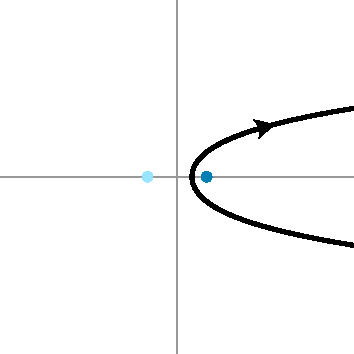
\includegraphics{figures/zeta_contour_3.pdf} \\[1em]
{\small The contour $\gamma_1$ in the $\zeta$ plane.}
\end{center}

It happens\footnote{\textcolor{magenta}{Veronica:} This comes from \cite[equation~15.4.14]{dlmf}.} that for our desired branch of $u$,
\[ \frac{1}{4u^2 - 1} = -F\big(\tfrac{1}{3}, \tfrac{2}{3}; \tfrac{1}{2}; \zeta^2\big), \]
so we can rewrite integral~\ref{integral:mod-bessel-zeta} as
\[ K = \frac{1}{i\sqrt{3}} \int_{\gamma_z} e^{-z\zeta} F\big(\tfrac{1}{3}, \tfrac{2}{3}; \tfrac{1}{2}; \zeta^2\big)\;d\zeta. \]
This gives us an alternate route to the conclusion of Section~\ref{spatial}, which we'll follow below.

In addition to the solutions $g_1$ and $f_0$ from Section~\ref{spatial-success}, equation~\ref{eqn:hypergeom} has the solutions
\begin{alignat*}{2}
g_0 &\;=\;& & F\big(\tfrac{2}{3}, \tfrac{4}{3}; \tfrac{3}{2}; 1-\xi\big) \\
f_1 &\;=\;& (1-\xi)^{-1/2} & F\big(\tfrac{1}{6}, \tfrac{5}{6}; \tfrac{1}{2}; 1-\xi\big),
\end{alignat*}
given by formulas 15.10.13 and 15.10.14 from \cite{dlmf}.

The quadratic transformation identity 15.8.27 from \cite{dlmf} shows \textcolor{magenta}{[verified numerically]} that\footnote{Note that $2\Gamma(\tfrac{1}{2})\Gamma(\tfrac{3}{2}) = 2\Gamma(\tfrac{1}{2})\,\tfrac{1}{2}\Gamma(\tfrac{1}{2}) = \pi$ and $\big[\Gamma(\tfrac{5}{6})\Gamma(\tfrac{7}{6})\big]^{-1} = \big[\Gamma(\tfrac{5}{6})\,\tfrac{1}{6}\Gamma(\tfrac{1}{6})\big]^{-1} = \frac{6\sin(\tfrac{1}{6} \pi)}{\pi} = \frac{3}{\pi}$.}
\[ F\big(\tfrac{1}{3}, \tfrac{2}{3}; \tfrac{1}{2}; \zeta^2\big) = \tfrac{1}{3}(g_1 + g_0), \]
so we have
\[ K = \frac{1}{i\,3\sqrt{3}} \int_{\gamma_z} e^{-z\zeta} (g_1 + g_0)\;d\zeta. \]
The solution $g_1$ is holomorphic on $\zeta \in [1, \infty)$, so it integrates to zero. The solution $g_0$, in contrast, is non-meromorphic at $\zeta = 1$. Along the branch cut $\zeta \in [1, \infty)$, its above-minus-below difference is $-\tfrac{3\sqrt{3}}{2}\,f_0$,
as given\footnote{Note that $\Gamma(\tfrac{3}{2}) \Gamma(\tfrac{1}{2})^{-1} = \tfrac{1}{2}$ and $\big[\Gamma(\tfrac{2}{3})\Gamma(\tfrac{4}{3})\big]^{-1} = \big[\Gamma(\tfrac{2}{3})\,\tfrac{1}{3}\Gamma(\tfrac{1}{3})\big]^{-1} = \frac{3\sin(\tfrac{1}{3} \pi)}{\pi} = \frac{3\sqrt{3}}{2\pi}$.} by equation~15.2.3 from \cite{dlmf}.
Hence,
\begin{align*}
K & = \frac{i}{2} \int^\infty_1 e^{-z\zeta} f_0\;d\zeta \\
e^z K & = \frac{i}{2} \int^\infty_1 e^{-z(\zeta - 1)} f_0\;d\zeta \\
K_1 & = \tfrac{i}{2} \laplace_{\zeta_1} f_0,
\end{align*}
just as we found in Section~\ref{spatial-success}.
\subsection{Another solution}
Section~\ref{contour-argument} associates the solution $K$ of equation~\ref{eqn:mod-bessel} with the solution $g_0$ of equation~\ref{eqn:hypergeom}, which contributes the pole at $\zeta = 1$ of
\[ \frac{du}{d\zeta} = \frac{1}{4u^2 - 1} = \tfrac{1}{3}(g_1 + g_0). \]
The solution $g_1$, which contributes the pole at $\zeta = -1$, is associated with another solution of equation~\ref{eqn:mod-bessel}.

To express this other solution as a Laplace transform, following the method of Section~\ref{spatial-success}, we would use the solution
\[ f_1 = (1-\xi)^{-1/2} F\big(\tfrac{1}{6}, \tfrac{5}{6}; \tfrac{1}{2}; 1-\xi\big) \]
of equation~\ref{eqn:hypergeom}, given by formula~15.10.14 from \cite{dlmf}. This is the only solution, up to scale, which has a fractional power singularity at $\zeta = -1$.

In summary, the contour integration method of solving equation~\ref{eqn:mod-bessel} is associated with the basis
\begin{align*}
g_1 & = F\big(\tfrac{2}{3}, \tfrac{4}{3}; \tfrac{3}{2}; \xi\big) \\
g_0 & = F\big(\tfrac{2}{3}, \tfrac{4}{3}; \tfrac{3}{2}; 1-\xi\big)
\end{align*}
of solutions for equation~\ref{eqn:hypergeom}, given by formulas 15.10.11 and 15.10.13 from \cite{dlmf}. These solutions contribute the poles at $\xi = 1$ and $\xi = 0$, respectively, of a generic solution.

The Laplace transformation method of solving equation~\ref{eqn:mod-bessel}, on the other hand, is associated with the basis
\begin{alignat*}{2}
f_1 &\;=\;& (1-\xi)^{-1/2} & F\big(\tfrac{1}{6}, \tfrac{5}{6}; \tfrac{1}{2}; 1-\xi\big) \\
f_0 &\;=\:& \xi^{-1/2} & F\big(\tfrac{1}{6}, \tfrac{5}{6}; \tfrac{1}{2}; \xi\big)
\end{alignat*}
given by formulas 15.10.14 and 15.10.12 from \cite{dlmf}. These solutions, up to scale, are the only ones with fractional power singularities.

Identities 15.10.18, and 15.10.22 from \cite{dlmf} give the change of basis
\begin{alignat*}{3}
f_1 &\;=\;&\tfrac{1}{\sqrt{3}}\,g_1 &\;+\;& \tfrac{1}{2}\,f_0 \\
f_0 &\;=\;& \tfrac{1}{\sqrt{3}}\,g_0 &\;+\;& \tfrac{1}{2}\,f_1.
\end{alignat*}
Summing these identities, we see that
\[ g_1 + g_0 = \tfrac{\sqrt{3}}{2}\,(f_1 + f_0), \]
giving the alternate decomposition
\[ \frac{du}{d\zeta} = \tfrac{1}{2\sqrt{3}}\,(f_1 + f_0). \]
\subsection{Lifting to a countable cover}
Formula~\ref{integral:mod-bessel-rational} expresses the modified Bessel function $K_{m/n}$ as an exponential integral on a finite cover of $\C$. Lifting to a countable cover reveals this formula as a special case of a general integral formula for modified Bessel functions.

Setting $u = \cosh(t/n)$ and recalling that
\begin{align*}
\cosh(n\tau) & := T_n(\cosh(\tau)) \\
\sinh(m\tau) & := U_{m-1}(\cosh(\tau)) \sinh(\tau),
\end{align*}
we can rewrite formula~\ref{integral:mod-bessel-rational} as \textcolor{magenta}{[switching to the conventional sign for the projection map, so $\Lambda^{(3)}$ now comes from $\infty$ at $-60^\circ$ and goes to $\infty$ at $60^\circ$]}
\begin{align}
\notag K_{m/n}(z) & = \frac{n}{2 \sinh\big(\tfrac{m}{n}\,i\pi\big)} \int_{z^{-\textcolor{DarkCyan}{1/n}}\Lambda^{(k)}} \exp\left[z T_n(u)\right]\,U_{m-1}(u)\,du \\
\notag & = \frac{n}{2 \sinh\big(\tfrac{m}{n}\,i\pi\big)} \int_{\textcolor{magenta}{\Omega}} \exp\left[z \cosh(t)\right]\,U_{m-1}(\cosh(t/n))\,\sinh(t/n)\,d(t/n) \\
\label{integral:mod-bessel-lifted} & = \frac{n}{2 \sinh\big(\tfrac{m}{n}\,i\pi\big)} \int_{\textcolor{magenta}{\Omega}} \exp\left[z \cosh(t)\right]\,\sinh\big(\tfrac{m}{n}\,t\big)\,dt.
\end{align}
For any $\nu \in \C \smallsetminus \Z$, formulas~10.27.4 and 10.32.12 from \cite{dlmf} tell us that
\begin{align}
\notag K_\nu(z) & = \frac{\pi}{\sin(\nu \pi)} \cdot \frac{1}{2}\big[ I_{-\nu}(z) - I_\nu(z) \big] \\
\notag & = \frac{1}{2i \sin(\nu \pi)} \int_\Omega \exp\left[z \cosh(t)\right]\,\frac{1}{2}\left[e^{\nu t} - e^{-\nu t}\right]\,dt \\
\label{intgral:mod-bessel-general} & = \frac{1}{2 \sinh(\nu\,i\pi)} \int_\Omega \exp\left[z \cosh(t)\right]\,\sinh(\nu t)\,dt,
\end{align}
where $\Omega$ is a path that comes from $\infty$ along $-i \pi + (0, \infty)$ and goes to $\infty$ along $i \pi + (0, \infty)$. The integral converges when $z$ is in the right half-plane. We get formula~\ref{integral:mod-bessel-lifted} when we choose a rational parameter $\nu = m/n$.

When $\nu$ goes to $0$, formula~\ref{integral:mod-bessel-lifted} becomes
\[ K_\nu(z) = \frac{1}{2\pi i} \int_\Omega \exp\left[z \cosh(t)\right]\,t\,dt. \]
Choosing $\Omega$ to be the unit-speed path that runs from $\infty$ leftward to $-i\pi$, upward to $i\pi$, and rightward back to $\infty$, we can rewrite this formula as
\begin{align*}
K_\nu(z) & = \frac{1}{2\pi i} \int_0^\infty \exp\left[-z \cosh(t)\right]\,2\pi i\,dt \\
& = \int_0^\infty \exp\left[-z \cosh(t)\right]\,dt \\
& = \int_1^\infty \exp\left[-z\,\tfrac{1}{2}\left(s + \tfrac{1}{s}\right)\right]\,\frac{ds}{s},
\end{align*}
with $s = e^t$. This is a special case of formula~10.32.9 from \cite{dlmf}.
\subsection{Correspondence with Mari\~{n}o's series}
Let $F_1(z)$ be the holomorphic function corresponding to Mari\~{n}o's formal power series $\varphi_1(z^{-1})$. The formal power series corresponding to $F_1$ will be written in the variable $z$.

\begin{align*}
\Ai(x) & = \tfrac{1}{2\sqrt{\pi}} x^{-1/4} e^{-z} \varphi_1\big(\tfrac{2}{3} z^{-1}\big) \\
& = \tfrac{1}{2\sqrt{\pi}} x^{-1/4} e^{-z} F_1\big(\tfrac{3}{2} z\big) \\
\Ai(x) & = \frac{1}{\pi\sqrt{3}} x^{1/2} K(\tfrac{2}{3} x^{3/2})
\end{align*}
Putting together,
\begin{align*}
\tfrac{1}{2\sqrt{\pi}} x^{-1/4} e^{-z} F_1\big(\tfrac{3}{2} z\big) & = \frac{1}{\pi\sqrt{3}} x^{1/2} K(\tfrac{2}{3} x^{3/2}) \\
\tfrac{\sqrt{3\pi}}{2}\;x^{-3/4} e^{-z} F_1\big(\tfrac{3}{2} z\big) & = K(\tfrac{2}{3} x^{3/2}) \\
\tfrac{\sqrt{3\pi}}{2}\;\big(\tfrac{3}{2} z)^{-1/2} e^{-z} F_1\big(\tfrac{3}{2} z\big) & = K(z) \\
\sqrt{\tfrac{\pi}{2}}\;z^{-1/2} e^{-z} F_1\big(\tfrac{3}{2} z\big) & = K(z) \\
\sqrt{\tfrac{\pi}{2}}\;\big[\laplace^{-1} z^{-1/2}\big] * \big[\laplace^{-1} F_1\big(\tfrac{3}{2} z\big)\big](\zeta - 1) & = k(\zeta) \\
\sqrt{\tfrac{\pi}{2}}\;\left[\Gamma\big({-\tfrac{1}{2}}\big)^{-1} \zeta^{-1/2}\right] * \tfrac{2}{3} f_1\big[\tfrac{2}{3}(\zeta - 1)\big] & = k(\zeta) \\
-\tfrac{1}{3\sqrt{2}}\;\left[\zeta^{-1/2}\right] * f_1\big[\tfrac{2}{3}(\zeta - 1)\big] & = k(\zeta) \\
\end{align*}
Notice that if the hypergeometric differentiation formula holds for fractional derivatives,
\[ \big(\tfrac{\partial}{\partial \xi}\big)^{1/2}F\big(\tfrac{2}{3}, \tfrac{4}{3}; \tfrac{3}{2}; \xi\big) \propto F\big(\tfrac{7}{6}, \tfrac{11}{6}; 2; \xi\big) \]
\bibliographystyle{utphys}
\bibliography{airy-resurgence}
\end{document}